%! Author = Frederik Bußmann
%! Date = 22.06.2023

\section{Analyse und Konzept} \label{sec:03-concept}

Im folgenden Kapitel werden verschiedene Techniken zur kontinuierlichen Integrierung von Code analysiert und eine
Konzeption für Shopware-basierte Projekte erarbeitet.
Zunächst wird die aktuelle Situation untersucht und eine Grundlage für die Einführung von Qualitätsanalyse-Tools und
automatisiertem Testing gelegt.
Anschließend werden verschiedene \acrshort{ci}-Tools analysiert und für den Einsatz in der zu konzipierenden Pipeline
bewertet.
Zuletzt wird eine Konzeption durchgeführt, diese stützt sich dabei auf die zuvor festgelegte Ausgangssituation und die
untersuchten Tools.

\subsection{Analyse der Ausgangssituation} \label{subsec:03-concept-1}

Die aktuelle Situation stellt sich wie folgt dar: Es gibt verschiedene Kunden, die mit unterschiedlichen Versionen von
Shopware arbeiten.
Diese Kunden sind bei verschiedenen Hosting-Anbietern untergebracht, was zu einer Vielfalt an technischen Umgebungen
führt, in denen die Software betrieben wird.
Darüber hinaus verwendet jeder Kunde eine individuelle Kombination aus Plugins und Eigenentwicklungen, die auf seine
spezifischen Bedürfnisse zugeschnitten sind.
Diese Diversität stellt eine Herausforderung dar, da sie eine Vielzahl von Variablen in die Entwicklung und Wartung der
Software einbringt.
Um eine generalisierte Strategie erstellen zu können, wird sich also zunächst auf die Gemeinsamkeiten von
Shopware-Projekten konzentriert.
\begin{figure}[H]
    \centering
    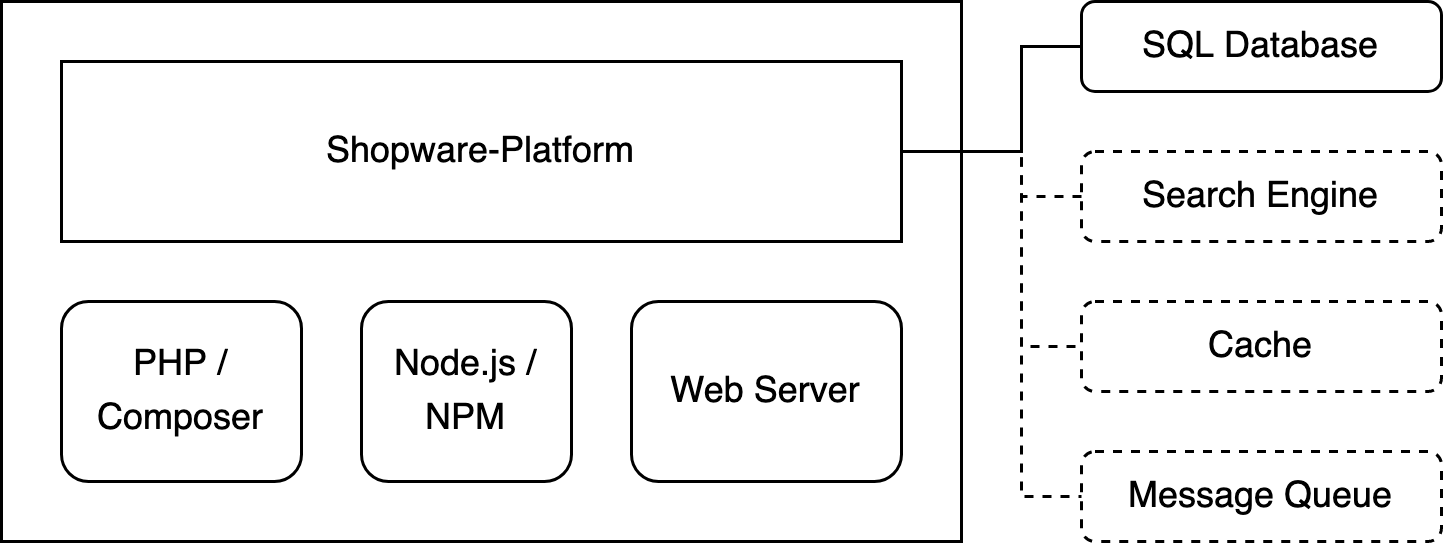
\includegraphics[width=0.6\textwidth]{images/content/shopware-requirements}
    \captioncite[Eigene Darstellung nach]{shopware-requirements}{Umgebung und Abhängigkeiten der Shopware-Platform}
    \label{fig:shopware-requirements}
\end{figure}
Shopware besteht aus einer Vielzahl von Verzeichnissen und Dateien, jede Version der Software und jedes
Shopware-basierte Projekt unterscheiden sich voneinander.
Ungeachtet von Projekt und Version gibt es jedoch einige Grundvoraussetzungen für das Ausführen von Shopware.
Die Programmiersprache PHP mit einigen Extensions und der Paketmanager Composer müssen in der ausführenden Umgebung
installiert sein.
Zusätzlich wird die Javascript-Runtime \glqq Node\grqq\ mit Paketmanager \acrshort{npm} benötigt, um das Frontend zu
bauen.
Die Software setzt außerdem eine Datenbank für den Betrieb des Shops und das Durchführen von End-to-End-Tests voraus,
und benötigt einen Webserver um aufgerufen werden zu können.
Im Live-Betrieb unterstützt die Plattform das optionale Anbinden einer Message-Queue und einer Search Engine, um viele
gleichzeitige Zugriffe von Usern verwalten zu können und das Suchen von Produkten und Herstellern für Shop-Kunden zu
ermöglichen.
Zur weiteren Optimierung der Produktions-Umgebung kann zudem ein Cache für Warenkorb-Inhalte und Nutzer-Sessions
eingeführt werden.
\footpartcite{shopware-requirements}
In Abbildung\ \ref{fig:shopware-requirements} werden die Abhängigkeiten der Shopware-Platform und die verschiedenen
Services für den Betrieb der Software aufgezeigt.
Um ein Projekt installieren und ausführen zu können, oder um Tests auf der Code-Base durchzuführen, wird also eine
Umgebung vorausgesetzt, in der die benötigten Services und Tools installiert sind.

\subsection{Auswertung von CI/CD-Tools} \label{subsec:03-concept-2}

Um die Konzeption einer \acrshort{ci}-Pipeline durchführen zu können, müssen zunächst die zur Umsetzung verfügbaren
Tools erfasst und für den Einsatz in Kundenprojekten bewertet werden.
Dabei spielen verschiedene Aspekte eine Rolle, wie die Kompatibilität mit dem bestehenden Technologie-Stack, die
Skalierbarkeit und die Benutzerfreundlichkeit.
Nachfolgend werden verschiedene Kategorien von Tools und Services die für eine \acrshort{ci}-Pipeline genutzt werden
können, vorgestellt.

\subsubsection{Version Control Systems}

Die Integration von Software wird durch \acrshort{vcs} ermöglicht.
Änderungen im Code werden hier hinzugefügt und verschiedene Versionsstände zusammengeführt.
\acrshort{vcs} somit ein integraler Bestandteil von Continuous Integration, Fowler setzt das Führen eines einzelnen
Source-Repositories voraus, welches die Software, inklusive aller Build- und Testing-Dateien, verwaltet.
\footpartcite{fowler}
Um eine vollumfängliche \acrshort{ci}-Strategie erstellen zu können, muss also die Versionskontroll-Software
inklusive dazugehöriger Services berücksichtigt werden.
Für die Konzeption wurden einige Bekannte und erprobte Anbieter von Enterprise-\acrshort{vcs} untersucht:

\begin{itemize}
    \item{
        \textbf{GitHub:}\par
        GitHub ist ein webbasierter Hosting-Service für Versionierung mit Git.
        Es bietet alle verteilten Versionskontroll- und Quellcodeverwaltungsfunktionen von Git sowie einige
        eigene Funktionen.
        Es bietet Zugriffskontrolle und mehrere Kollaborationsfunktionen wie Aufgabenverwaltung, Fehlerverfolgung und
        Feature-Requests für Projekte.
        GitHub bietet sowohl Pläne für private Repositorys als auch kostenlose Konten, die normalerweise verwendet
        werden, um Open-Source-Softwareprojekte zu hosten.
        Der Service bietet außerdem \acrshort{ci}-Tools und Pipeline-Verwaltung an.
        Als Managed Service kümmert sich GitHub um die Wartung der Infrastruktur.\footpartcite{github}
    }

    \item{
        \textbf{GitLab:}\par
        GitLab ist ein webbasiertes \acrshort{vcs}-Tool, welches einen Git-Repository-Manager bereitstellt.
        Der Service ist vergleichbar mit GitHub und bietet viele ähnliche Funktionen, wie Issue-Tracking,
        kontinuierliche Integration und Deployment-Pipelines, sowie eine integrierte Wiki-Funktion für die
        Dokumentation.
        Es wird unter einer Open-Source-Lizenz vertrieben und eine Self-Managed-Version ermöglicht es,
        GitLab auf eigenen Servern zu installieren und zu verwalten.
        Dies bietet mehr Kontrolle über die Daten und die Möglichkeit, die Plattform an spezifische Bedürfnisse
        anzupassen.\footpartcite{gitlab}
    }

    \item{
        \textbf{Bitbucket:}\par
        Bitbucket ist ein weiteres webbasiertes Tool zur Verwaltung von \acrshort{vcs}, welches sowohl von
        kommerziellen als auch von kostenlosen Konten genutzt wird.
        Es wird von der Firma Atlassian betrieben und ermöglicht das Hosting von Git- und Mercurial-Repositorys.
        Bitbucket integriert auch mit anderen Atlassian-Produkten wie Jira und Confluence.
        Es bietet Funktionen wie Pull-Requests für Code-Reviews und Inline-Kommentare.
        Bitbucket bietet sowohl Managed als auch Self-Hosted-Optionen.\footpartcite{bitbucket}
    }

    \item{
        \textbf{SourceForge:}\par
        SourceForge ist eine Open-Source \acrshort{vcs}-Lösung, welche sowohl Git als auch Mercurial unterstützt.
        Die Plattform kann sowohl zur Versionskontrolle als auch für das Ausliefern von Software verwendet werden,
        wobei diese oft für Open-Source-Projekte genutzt wird.
        SourceForge ist webbasiert und bietet den direkten Download von einer Vielzahl von Software-Projekten an.
        \footpartcite{sourceforge}
    }
\end{itemize}

\subsubsection{Pipeline- und Test-Runners}

Um die in einer Versionskontroll-Software eingeführten Code-Änderungen automatisiert bauen, testen und ausliefern zu
können, wird eine ausführende Umgebung für diese Prozesse benötigt.
Für diese Problemstellung gibt es Pipelines, welche zum Ausführen von Befehlen und Prozessen zur automatischen
Integration und dem Testen von Code genutzt werden.\footpartcite[2571]{benefits-challenges}
Pipelines spielen durch das kontinuierliche Integrieren von entwickeltem Code eine integrale Rolle bei der Reduzierung
der Cycle Time\footpartcite{fowler} und sind somit wichtig zum Erreichen des Ziels $Z_1$ der Arbeit.
Große Enterprise-\acrshort{vcs}-Anbieter wie GitHub, GitLab und Bitbucket haben bereits eine Pipeline-Lösung in ihrem
System integriert und bieten Hardware-Ressourcen zum Ausführen der Pipelines an.
Neben den eingebauten Pipeline-Services der Enterprise-Anbieter gibt es einige eigenständige Tools, welche Teils selbst
gehostet werden müssen.
Nachfolgend werden einige dieser \acrshort{ci}/\acrshort{cd}-Services im Hinblick auf den Einsatz in der zu
entwickelnden Strategie untersucht:

\begin{itemize}
    \item{
        \textbf{GitHub Actions:}\par
        GitHub Actions ist die eingebaute \acrshort{ci}/\acrshort{cd}-Lösung von GitHub.
        Actions können in jedem Repository in einem bestimmten Verzeichnis in Form von Konfigurations-Dateien im
        \acrshort{yaml}-Format angelegt werden.
        Durch Actions kann an verschiedenen Stellen im Nutzungszyklus des \acrshort{vcs} angeknüpft werden, um zum
        Beispiel nach einem Push oder bei Merge-Prozessen verschiedene Aktionen mit dem eingeführten Code durchzuführen.
        An dieser Stelle können dann je Branch verschiedene Aktionen definiert werden, wie zum Beispiel das Durchführen
        von Build-Prozessen, Tests und des Software-Deployments.
        Beim Merging-Prozess von verschiedenen Branches kann so zum Beispiel das erfolgreiche Durchlaufen der Pipeline
        vorausgesetzt werden, um fehlerhaften oder ungetesteten Code im Ziel-Branch zu vermeiden.
        Die für das Ausführen der Pipeline benötigten Umgebungsvariablen, Passwörter und andere vertrauliche Daten
        können dabei in einer von GitHub zur Verfügung gestellten, sicheren Datenbank verwaltet werden.
        \footpartcite{github-actions}
    }

    \item{
        \textbf{GitLab CI/CD:}\par
        Ähnlich wie GitHub bietet auch GitLab eine eingebaute Pipeline-Lösung für das Ausführen von \acrshort{ci}- und
        \acrshort{cd}-Prozessen.
        GitLab CI/CD ist vollständig in GitLab integriert und verwendet eine Konfigurations-Datei innerhalb des
        Repositories, um die Phasen des \acrshort{ci}/\acrshort{cd}-Prozesses zu definieren.
        Es bietet eine breite Palette von Funktionen, einschließlich der Parallelisierung von Tests, Pipelines für Merge
        Requests und das Verwalten von Umgebungsvariablen.
        GitLab CI/CD kann auf eigenen Servern oder in der Cloud ausgeführt werden, und sowohl für bei GitLab, als auch
        für extern gehostete Repositorys verwendet werden, was es zu einer flexiblen Lösung macht.
        \footpartcite{gitlab-ci-cd}
    }

    \item{
        \textbf{Bitbucket Pipelines:}\par
        Bitbucket bietet, ähnlich wie GitHub und GitLab, eine integrierte \acrshort{ci}/\acrshort{cd}-Lösung.
        Bitbucket Pipelines ermöglicht die Automatisierung von Build-, Test-/\acrshort{qa}- und Deployment-Prozessen und
        ist dabei direkt an das Repository angebunden.
        Der Service verwendet ebenfalls eine \acrshort{yaml}-Datei zur Konfiguration der Pipelines und bietet eine
        Vielzahl von vordefinierten Umgebungen und Integrationen mit anderen Tools.
        Wie GitLab, unterstützt auch Bitbucket Pipelines das parallele Durchführen von Tests.
        Pipelines können sowohl innerhalb von Bitbucket, als auch in der selbst-gehosteten Version genutzt werden.
        \footpartcite{bitbucket-pipelines}
    }

    \item{
        \textbf{Jenkins:}\par
        Jenkins ist ein Open-Source-Tool, das für Continuous Integration entwickelt wurde, aber auch Continuous Delivery
        unterstützt.
        Es bietet eine große Anzahl von Plugins und Erweiterungen, die es zu einer flexiblen Lösung für
        \acrshort{ci}/\acrshort{cd}-Pipelines machen.
        Jenkins unterstützt das Verteilen von Arbeitslast auf verschiedene Systeme und kann auf einer Vielzahl von
        Plattformen und Umgebungen ausgeführt werden.
        Der Service kann durch Plugins angepasst und erweitert werden, um eigene Build-, Testing- und
        \acrshort{qa}-Tools einführen zu können.
        Jenkins muss selbst gehostet werden, was eine größere Kontrolle über die Ausführungsumgebung ermöglicht, aber
        auch einen höheren Wartungsaufwand mit sich bringt.\footpartcite{jenkins}
    }

    \item{
        \textbf{Travis CI:}\par
        Travis CI ist ein Cloud-basierter \acrshort{ci}/\acrshort{cd}-Service, der sich besonders gut für Projekte
        eignet, die auf GitHub gehostet werden.
        Es bietet eine einfache Einrichtung und Konfiguration durch eine \acrshort{yaml}-Datei im Repository und
        unterstützt eine Vielzahl von Programmiersprachen und Tools.
        Der Service ermöglicht das gleichzeitige Testen in verschiedenen Umgebungen und die Verwaltung von
        Umgebungsvariablen und Secrets, sowie das Erweitern der Plattform für die Integration externer Applikationen.
        Travis CI bietet sowohl kostenlose Pläne für Open-Source-Projekte als auch kostenpflichtige Pläne für private
        Projekte.
        \footpartcite{travis-ci}
    }
\end{itemize}

\subsubsection{Testing-Tools}

Shopware-Projekte gewinnen schnell an Umfang, der Aufwand für das manuelle Testen der einzelnen Entwicklungen steigt mit
jedem eingeführten Feature.
Software-Tests sind ein nützliches Tool für \acrshort{ci}-Pipelines und helfen dabei, das aufwändige manuelle Testen
der einzelkomponenten bei einem Software-Release zu minimieren.
Automatisierte Tests werden eingesetzt, um sicherzustellen, dass mit neuen Features weniger Wechselwirkungen mit vorher
eingeführter Logik aufkommen und um Fehler im Entwicklungsprozess früher entdecken zu können.
Das häufige, automatisierte Testing in der \acrshort{ci} kann sich positiv auf die Qualität der entwickelten
Software auswirken
\footpartcite[281]{test-driven-development}\textsuperscript{,\ }\footpartcite[2570]{benefits-challenges}, somit sind
Software-Tests im Hinblick auf Zielsetzung $Z_2$ der Arbeit relevant.
Nachfolgend werden verschiedene Arten von Software-Tests beschrieben und Tools für das Einbinden dieser Tests in der
bestehenden Systemlandschaft untersucht:

\begin{itemize}
    \item {
        \textbf{Unit-Tests:}\par
        Unit-Tests verifizieren das Verhalten von kleinen Elementen eines Software-Systems, meist einzelner Klassen.
        Beim Durchführen von Unit-Tests wird das gewünschte Verhalten von Software-Komponenten definiert und
        diese anschließend ausgeführt um das Ergebnis mit dem zuvor definierten, erwarteten Verhalten zu vergleichen.
        Diese Tests haben keine äußerlichen Abhängigkeiten wie Datenbanken, da der jeweils getestete Code isoliert
        vom Rest des Software-Systems getestet wird.
        Um etwaige Abhängigkeiten die zur Ausführung des Codes benötigt werden zu umgehen, werden Mocks eingesetzt.
        Ein Mock stellt eine Nachahmung der Vorgehensweise einer Abhängikeit dar, so kann zum Beispiel das Verhalten
        einer Datenbank simuliert werden, ohne diese als Service im Testing-Prozess zu benötigen.
        Oftmals wird der Anteil von durch Tests abgedeckten Klassen und Funktionen im Kontrast zu der Anzahl an
        ungetesteten Komponenten der Software gemessen, dieser Wert wird als Coverage bezeichnet.
        \footpartcite[132--133]{duvall}
        Nachfolgend werden Tools für das Auführen von Unit-Tests in Shopware-basierten Projekten untersucht:

        \begin{itemize}
            \item {
                \textbf{PHPUnit:}\par
                PHPUnit ist ein weit verbreitetes Open-Source Unit-Testing-Framework, welches zum Erstellen von
                Unit-Tests in PHP-basierten Applikationen verwendet wird.
                Das Framework ermöglicht das Erstellen von Mocks und das Auswerten der Test-Coverage für das zu
                testende Projekt.
                \footpartcite{phpunit}
            }

            \item {
                \textbf{Jest:}\par
                Jest ist ein Javascript Testing-Framework und ermöglicht das Einbringen von Unit-Tests in
                JavaScript-basierten Applikationen.
                Ähnlich wie PHPUnit, unterstützt Jest das Erstellen von Mocks und bietet Funktionen zur Coverage an.
                Das Framework parallelisiert laufende Tests, um eine möglichst hohe Performance zu bieten.
                \footpartcite{jest}
            }
        \end{itemize}
    }

    \item {
        \textbf{Functional Tests:}\par
        Funktionstests stellen eine Umgebung dar, in der das Software-System auf Interoperatibiliät der
        einzelnen Komponenten und Services geprüft wird.
        Hierbei stehen alle Abhängigkeiten und Services für die Software zur Verfügung, um das Zusammespiel von
        verschiedenen Komponenten des Systems aus Sicht des Kunden zu testen.
        Diese Tests erfordern oft ein längeres Test-Setup und eine höhere Laufzeit.
        \footpartcite[136-138]{duvall}
        Im Folgenden werden einige Testing-Tools für systemweite Tests untersucht:

        \begin{itemize}
            \item {
                \textbf{Cypress:}\par
                Cypress ist ein Testing Framework für Webapplikationen.
                Es ermöglicht das automatisierte Testen von Benutzerinteraktionen innerhalb einer Webapplikation in
                einem realen Browser.
                Cypress ist besonders nützlich für das Testen von komplexen Webapplikationen und unterstützt sowohl
                Unit- als auch Integrations- und End-to-End-Tests.
                Cypress ermöglicht das Testen des Zusammenspiels des gesamten Projekts und kann zur automatisierung
                von Testfällen genutzt werden, bei denen normalerweise Nutzer-Interaktion erforderlich ist.
                \footpartcite{cypress}
            }

            \item {
                \textbf{Selenium:}\par
                Selenium ist ein weit verbreitetes Open-Source-Tool für automatisierte Tests.
                Ähnlich wie Cypress, ermöglicht es das Testen von Webanwendungen in verschiedenen Browsern und auf
                verschiedenen Plattformen.
                Selenium unterstützt eine Vielzahl von Programmiersprachen, darunter JavaScript, Java, C\#, Python und
                Ruby.
                Es kann als Testing-Tool in einem Web-basierten Projekt oder als automatisierungs-Tool für andere
                Aufgaben verwendet werden.
                \footpartcite{selenium}
            }
        \end{itemize}
    }

    \item {
        \textbf{Mutation-Tests:}\par
        Mutation Testing ist eine Testtechnik, bei der die Effektivität eines existierenden Testsets bestimmt werden
        kann.
        Hierbei wird der zu testende Source-Code verändert, oder mutiert, und dieser abgeänderte Code mit einem
        bestehenden Test-Set geprüft.
        Wenn die mutierte Variante des Codes durch das Test-Set aufgedeckt wurde, indem der Test fehlschlägt, wird
        der mutierte Code, auch Mutant genannt, als eliminiert betrachtet.
        Durch Mutation Tests können Schwachstellen in Software-Tests gefunden werden und die Qualität der bestehenden
        Tests eines Tests gemessen werden.
        Zur Messung der Effektivität eines Test-Sets wird der \glqq Mutation Adequacy Score\grqq\@ oder
        \glqq Mutation Score\grqq\ (\acrshort{ms}) genutzt.
        Schlägt der Test eines mutierten Quellcodes nicht fehl, wirkt sicht das negativ auf den \acrshort{ms} aus:
        \[MS = \frac{Anzahl\ eliminierter\ Mutanten}{Anzahl\ Mutanten}\]
        Das Ziel ist hierbei das Abdecken möglichst aller Mutanten durch ein Test-Set $T$, sodass dessen Mutation Score
        $MS = 1$ entspricht.\footpartcite[649--652]{mutation-testing}

        \begin{itemize}
            \item {
                \textbf{Infection:}\par
                Infection ist eine Mutation-Testing-Library für PHP.
                Sie ändert den Quellcode automatisch und führt dann bestehende Tests erneut aus, um zu sehen, ob diese
                fehlschlagen.
                Wenn die Tests bestehen, obwohl der Code mutiert wurde, zeigt Infection diese Stellen im Code an, damit
                diese verbessert werden können.
                Infection nutzt einen eigenen \glqq Mutation Score Indicator\grqq\ (\acrshort{msi}), die Formel zur
                Berechnung des \acrshort{msi} ist wie folgt definiert:
                \[TotalDefeatedMutants = KilledCount + TimedOutCount + ErrorCount\]
                \[MSI = \left(\frac{TotalDefeatedMutants}{TotalMutantsCount}\right) * 100\]
                Neben dem \acrshort{msi} stellt Infection noch weitere Faktoren zum Bestimmen der Effektivität von
                Test-Sets bereit.
                Die Library unterstützt die Integration mit PHPUnit, Codeception und weiteren Testing-Tools.
                \footpartcite{infection}
            }
        \end{itemize}
    }
\end{itemize}

\subsubsection{Static-Code-Analysis-Tools}

Neben automatisiertem Testing ist das statische Analysieren des Codes ein weiterer wichtiger Aspekt für die
Qualitätskontrolle von Software in einer \acrshort{ci}-Umgebung.
Wobei Tests nur die Ergebnisse des Ausführens von Komponenten und Funktionen messen, können statische
Code-Analysis-Tools die Struktur des Codes und die Einhaltung von vorgegebenen Standards bewerten.
Eine laufende \acrshort{ci}-Pipeline kann so bei der Einführung von Code, welcher nicht dem vorgegebenen Coding-Standard
entspricht, abgebrochen werden.
Dies zwingt die Entwickler eines Projekts dazu, eine einheitliche Code-Struktur zu verwenden und kann das Einführen
von Fehlern verringern.
Außerdem können Static-Code-Analysis-Tools durch Warnungen dazu beitragen, dass unperformanter Code nicht in die
Produktions-Umgebung gerät.\footpartcite{static-analysis}
Da statische Code-Analyse die Qualität der entwickelten Software verbessern können, ist diese hilfreich für das
Erreichen des Ziels $Z_2$ der Arbeit.
Im Folgenden werden einige dieser Tools für die in Shopware-Projekten verwendeten Programmiersprachen PHP und JavaScript
gesammelt:

\begin{itemize}
    \item {
        \textbf{ESLint:}\par
        ESLint ist ein statisches Tool zur Analyse von JavaScript-Code.
        Das Tool ist sehr anpassbar und kann für das Entwickeln mit verschiedenen Frameworks und Libraries genutzt
        werden.
        Viele \acrshort{ide}s unterstützen ESLint und zeigen Analyse-Resultate bereits bei der Entwicklung im Editor
        an.
        Das Tool unterstützt außerdem das automatische Beheben von bestimmten Syntax-Fehlern mit einem eingebauten
        Kommandozeilenbefehl.\footpartcite{eslint}
    }

    \item {
        \textbf{Danger:}\par
        Danger ist ein statisches Analyse-Tool, welches direkt in \acrshort{vcs} angebunden werden kann.
        Das Tool läuft während des \acrshort{ci}-Prozesses und kann zur automatisierung von Code-Review-Aufgaben
        genutzt werden.
        Mit Danger können Warnungen und Fehler in der Pipeline geworfen werden, wenn Pull-Requests (\acrshort{pr}s) zu
        groß werden, kein Changelog-Eintrag für Änderungen angelegt wurde, Lockfiles nicht up-to-date sind, der PR
        unzugewiesen ist und vieles mehr.
        Die offizielle Ausführung der Software umfasst die Programmiersprachen JavaScript, Ruby, Kotlin, Python und
        Swift, wobei es auch eine unoffizielle PHP-Implementierung gibt.
        \footpartcite{danger-js}\textsuperscript{,\ }\footpartcite{danger-php}
    }

    \item {
        \textbf{PHP\_CodeSniffer:}\par
        PHP\_CodeSniffer (\acrshort{phpcs}) ist ein Set aus zwei Kommandozeilen-Befehlen für das Analysieren von PHP-
        und JavaScript-Code und von Cascading Style Sheets (\acrshort{css}) nach einem gegebenen Coding-Standard und für
        das automatische Korrigieren von Abweichungen dieses Standards.
        Das Tool kann mit vorgegebenen und eigens erstellten oder angepassten Regelsätzen betrieben werden.
        \footpartcite{php-codesniffer}
    }

    \item {
        \textbf{PHP Mess Detector:}\par
        PHP Mess Detector (\acrshort{phpmd}) ist eine Software die nach vorgegebenen Problemen und Unstimmigkeiten in
        PHP-Code sucht.
        Das Tool kann zum verhindern des Einführens von überflüssigen Variablen und Methoden, unoptimiertem Code und
        möglichen Fehlern in die Zielumgebung genutzt werden.
        \acrshort{phpmd} kann ergänzend zu Danger und \acrshort{phpcs} zur statischen Analyse von PHP-Code verwendet
        werden.\footpartcite{php-mess-detector}
    }

    \item {
        \textbf{PHPStan:}\par
        PHPStan ist ein weiteres \acrshort{qa}-Tool für das statische Analysieren von PHP-Code.
        Es konzentriert sich auf die Erkennung von Fehlern, die im laufenden Betrieb zu Problemen führen können, wie
        z.B. Aufrufe von nicht existierenden Methoden, ungenutzte Variablen, usw.
        PHPStan kann in den Entwicklungsprozess integriert werden, um die Codequalität kontinuierlich zu verbessern.
        \footpartcite{phpstan}
    }

    \item {
        \textbf{Deptrac:}\par
        Deptrac ist ein statisches Code-Analyse-Tool, das dabei hilft, die Architektur eines PHP-Projekts zu verstehen
        und zu überprüfen.
        Es stellt sicher, dass die Abhängigkeiten zwischen den Modulen eines Projekts den definierten Architekturregeln
        entsprechen.
        Deptrac kann in den Entwicklungsprozess integriert werden, um die Architektur des Projekts kontinuierlich zu
        überwachen und zu verbessern.\footpartcite{deptrac}
    }

    \item {
        \textbf{License checker:}\par
        License checker ist ein Tool, das die Lizenzen von Abhängigkeiten in einem Projekt überprüft.
        Es kann dabei helfen, Lizenzprobleme bei Plugins und Erweiterungen von Drittanbietern zu identifizieren und zu
        vermeiden.
        Das Tool ist in PHP geschrieben und konzentriert sich auf das Überprüfen von Composer-Abhängigkeiten.
        \footpartcite{license-checker}
    }

    \item {
        \textbf{Symfony security checker:}\par
        Der Symfony Security Checker ist ein Befehlszeilentool, das überprüft, ob die in einem Symfony-Projekt
        verwendeten Abhängigkeiten bekannte Sicherheitslücken aufweisen.
        Das Tool kann zusammen mit der Symfony-\acrshort{cli} oder als eigenständiges Software installiert werden und
        hilft dabei, PHP-Projekte kontinuierlich zu überwachen und sicher zu halten.
        \footpartcite{symfony-security-checker}
    }
\end{itemize}

\subsection{Konzeption der CI-Strategie} \label{subsec:03-concept-3}

Im Folgenden wird die Konzeption der \acrshort{ci}-Strategie für Kundenprojekte auf Basis der Shopware-Platform
durchgeführt.
Zunächst wird eine generelle Projekt-Struktur für die Strategie definiert, wobei besonderer Wert auf die
Kompatibilität mit unterschiedlichen Shopware-Projekten gesetzt wird.
Anschließend werden, anhand der im vorherigen Abschnitt untersuchten \acrshort{ci}/\acrshort{cd}-Tools, Pipelines für
verschiedene Branching-Strukturen und Projekt-Ansätze erarbeitet.
Zuletzt wird der Einsatz von Continuous Delivery und Deployment in der Strategie im Hinblick auf Shopware-Projekte
bewertet.

\subsubsection{Projekt-Struktur}

% Strukturierung des Projekts (Wo liegen CI-Files, wo Projekt-Files, was gibt es noch?)
% Branching-Strukturen

Die Verzeichnis-Struktur von Shopware 6 ist

\subsubsection{Pipelines}

% Aufbau der Pipelines | Commit-CI vs. Merge-CI (Mal mit E2E, mal ohne, je nach Build-Time)
% Auswahl der CI-Tools (GitLab mit Gitlab CI/CD + Unit/Mutation/E2E-Tests + Static analysis)

\subsubsection{Continuous Delivery \& Deployment}

% Continuous Delivery (nicht Continuous Deployment, da Develop-, Staging- und Live und Kunde muss abnahme machen und
% wegen Sicherheitsanforderungen an E-Commerce-Applikationen, bla bla)

\clearpage
